%
% master thesis
%
\documentclass[a4paper,12pt,onecolumn,oneside,openany]{book}
\usepackage{./thesis}
\usepackage[dvipdfmx]{graphicx}
\usepackage{cite}
\usepackage{enumerate}
\usepackage{mediabb}
\usepackage[fleqn]{amsmath}
\usepackage{titletoc}
\usepackage{color}
\usepackage{subfigure}
\usepackage{mathtools}

% subfigure: ����̕����T�C�Y
\renewcommand{\subcapsize}{\small}
%
%
%
\begin{document}
% setting ---
%\mojiparline{35}	% ��s�����蕶�����̎w��
\linesparpage{35}	% 1�y�[�W������s���̎w��
\thispagestyle{empty}
\begin{center}
  \vspace*{20mm}

  {\LARGE 平成27年度修士論文\\}

  \vspace{10mm}

  {\huge\bf Radio Environment Database considering Primary User Activity in Time Domain}

  \vspace{5mm}

  {\huge\bf プライマリユーザの時間的変化を考慮した\\電波環境データベース構築\\}

  \vspace{10mm}

  \begin{table}[h]
    \LARGE
    \begin{center}
      \begin{tabular}{ll}
        学生番号 & 1431019\\
        氏名 & 王 昊\\
        情報・通信工学専攻  & 情報通信システムコース\\
        主指導教員 & 藤井 威生 教授\\
        指導教員 & 山尾 泰 教授\\
        提出日 & 平成28年1月29日\\
      \end{tabular}
    \end{center}
  \end{table}

  \begin{table}[h]
    \Large
    \begin{center}
      \begin{tabular}{|c|c|c|}
        \hline
        \makebox[90pt][c]{専攻主任印} & \makebox[90pt][c]{主指導教員印}  & \makebox[90pt][c]{指導教員印} \\
        \hline
        &&\\
        &&\\
        &&\\
        &&\\
        \hline
      \end{tabular}
    \end{center}
  \end{table}
\end{center}

\clearpage
\thispagestyle{empty}
\begin{center}
  {\Large 修 士 論 文 の 和 文 要 旨}
  \renewcommand{\arraystretch}{1.5}
  \begin{table}[!h]

    \begin{tabular}{|c|c|c|c|}
      \hline
      研究科・専攻 & \multicolumn{3}{|c|}{大学院 情報理工学研究科 情報・通信工学専攻 博士前期課程}\\
      \hline
      \makebox[0.15\hsize][c]{氏    名} & \makebox[0.3\hsize][c]{王 昊} & \makebox[0.15\hsize][c]{学籍番号} & \makebox[0.3\hsize][c]{1431019} \\
      \hline
      論 文 題 目 \rule[-7mm]{0mm}{16mm} & \multicolumn{3}{|c|}{\parbox[c]{0.75\hsize}{Radio Environment Database considering Primary User Activity in Time Domain}} \\
      \hline
      \multicolumn{4}{|l|}{ 要  旨 } \\
      \multicolumn{4}{|l|}{\parbox[t]{\hsize}{
コグニティブ無線を用いた周波数共用において,周波数の二次利用者(SU: Secondary User) は既存の周波数割り当てユーザ(PU: Primary User) への干渉を回避する必要がある.その中で自身の通信品質を確保するためには,正確な電波環境推定技術が重要である.筆者らは,これまで車載無線機やスマートフォンといった移動端末が観測した膨大な電波環境情報から構築される電波環境データベースを提案してきた.テレビ帯域を対象とした実証実験により,従来の距離減衰モデルに基づく手法と比較してPU の平均受信電力値の空間的な分布を精度良く推定できることを明らかにしている.しかし,これまではPU の通信状態のON/OFF 遷移を考慮せずに観測値を一意に平均化していた.そのため,無線LAN のように観測期間内に状態遷移する可能性のあるシステムについては,最終的な平均結果とON 状態の平均受信電力値に差が生じる恐れがあった.そこで本稿では,PU の通信状態の遷移を検出するセンシング手法を提案する.提案手法では,電波環境データベースに蓄積された統計情報と連携し,協調センシングによって電波環境を観測することで状態遷移を検出する.本手法により,通信を行なっている状態での受信電力値の取り出しが可能となり,結果としてPU が通信を行なっている状態での平均受信信号電力値を精度良く推定できる.本稿では特に,状態遷移時間の検出に焦点を当てたシミュレーション評価を行ない,その有効性を示す.}} \\
      \multicolumn{4}{|l|}{}\\
      \multicolumn{4}{|l|}{}\\
      \multicolumn{4}{|l|}{}\\
      \multicolumn{4}{|l|}{}\\
      \hline
    \end{tabular}

  \end{table}
  \renewcommand{\arraystretch}{1.0}
\end{center}

% abstruct ---
        % ----------------------------
% Abstract (japanese)
% ----------------------------
%\clearpage
\pagenumbering{roman}
%\setcounter{page}{0}
\begin{jabstract}
近年,周波数の枯渇問題を解消するための抜本的な対策として,周波数共用におけるコグニティブ無線技術が活発に研究を行われている.コグニティブ無線を用いた周波数共用において,周波数の二次利用者(SU: Secondary User) は既存の周波数割り当てユーザ(PU: Primary User)への干渉を回避する必要がある.その中で自身の通信品質を確保するためには,正確な電波環境推定技術が重要である.従来研究では,本研究室がこれまで車載無線機やスマートフォンといった移動端末が観測した膨大な電波環境情報から構築される実測値に基づく電波環境データベースを提案してきた.テレビ帯域を対象とした実証実験により,従来の距離減衰モデルに基づく手法と比較してPUの平均受信電力値の空間的な分布を精度良く推定できることを明らかにしている.しかし,これまではPUの通信状態のON/OFF遷移を考慮せずに観測値を一意に平均化していた.そのため,無線LANやセルラ通信のように観測期間内に状態遷移する可能性のあるシステムについては,最終的な平均結果とON状態の平均受信電力値に差が生じる恐れがあった.そこで本研究では,観測期間内にPUの通信状態が時間的に遷移する場合の電波環境データベースの構築における精度について検討を行う.1回の観測期間内での受信電力に関する分布変化を検出することにより,PU の通信状態の遷移点を検出するアルゴリズムを提案する.その分布の変化検出にCUSUMアルゴリズムとGLRアルゴリズムが用いられ,2つの分布の累積対数確率密度比の変化傾向から遷移点の検出が可能となる.検出した遷移点を用いて,通信を行なっている状態のみの有効期間から受信電力値の取り出しが可能となり,PU が通信を行なっている状態での平均受信信号電力値を精度良く推定できる.本研究では特に,状態遷移の検出性能及び受信電力値の推定性能に焦点を当てたシミュレーション評価を行ない,その有効性を示す.シミュレーションにより,提案手法を用いることで遷移点が精度よく検出され,受信電力値の推定誤差が状態遷移が考慮されていない従来手法より抑えることが可能である.
\end{jabstract}
%
%
%
% ----------------------------
% Abstract (english)
% ----------------------------
\begin{abstract}
Recently, with the fast development of wireless communication technology, cognitive radio (CR) has been recognized as a promising solution to address the problem of impending spectrum scarity for improving the utilization of spectrum for various wireless applications. In a CR system, it allows the Secondary Users (SUs) to opportunistically utilize the temporal and/or spatial unused spectrum holes without harmful interference to Primary Users (PUs). While SUs can occupy avaliable spectrum holes as long as the corresponding PU is in active, they must immediately evacuate the band as soon as the corresponding PU appears. One of the main chanllenges is to intelligently determine ongoing PU activity to avoid interferece toward PU. SUs can evacuate the band without affecting PU’s activity and opportunistically access the spectrum to maximize the spectrum usage if the information about PU can be obtained in advance. Hence, more information about PU leads to more effective spectrum usage for SUs, and an external device for provding information of PU is necessary. In conventional database construction method, the activity of primary user is considered to be always ON when the sensor uses the spectrum sensing to calculate the received power at each place. However, a state transition may occur during the sensing period, which leads to a reliability degradation of the RED. In this thesis, an active period detection method of primary signal is proposed. In this method, transition point detection is used to detect a distribution change between ON and OFF state with applying CUSUM (cumulative sum) algorithm and GLR (Generalized Likelihood Ratio) algorithm, which the cumulative sum of log probability density ratio value is calculated to detect the change between two different distribution.  Then an active period is extracted by using the detected transition point. In this thesis, we focus on the transition point detection performance and received power detction performance. From simulation results, the transition point is well detected and the estimated received power is more accurate than the one using the conventional method.
\end{abstract}

% table of contents ---
\tableofcontents
% introduction --- 
\chapter[Introduction]{Introduction}
%\addcontentsline{toc}{chapter}{Chapter 1\\Introduction}
\label{chapter:introduction}
\pagenumbering{arabic}

In chapter \ref{chapter:introduction},  present spectrum scarcity problem as the background of this thesis and technology proposed for solution is described. Aslo, the overview of this thesis and purpose is described. 
\section{Background}
 Due to the rapid development of wireless communication systems, a demand on sprectrum resource for communication has increased explosively. Because the data rate and perfomance of the wireless communication system, such as mobile phone, are improved, it leads to a serious sprectrum scarcity problem.

 From Fig. \ref{fig:Cisco}, reference \cite{ref:Cisco} predicts that Global mobile data traffic will increase nearly tenfold between 2014 and 2019 and mobile data traffic will grow at a compound annual growth rate (CAGR) of 57 percent from 2014 to 2019, reaching 24.3 exabytes per month by 2019. 
\begin{figure}[!htp]
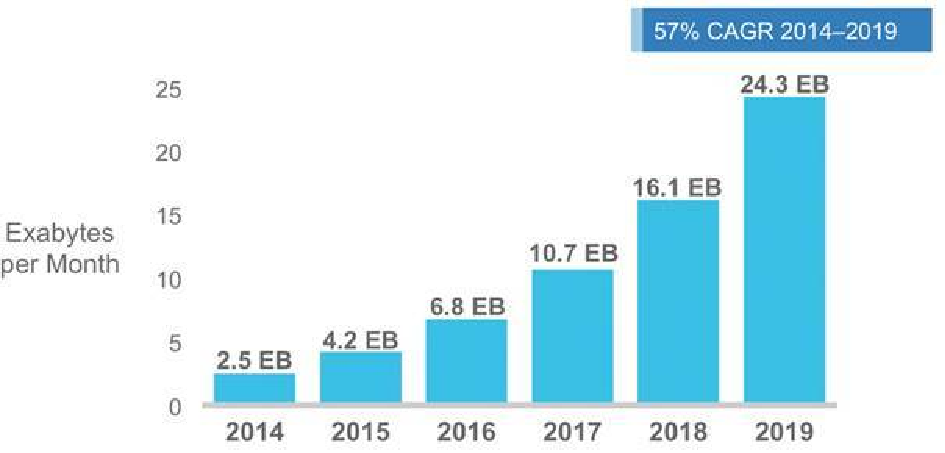
\includegraphics[width=150mm,clip]{traffic_trend.pdf}
\caption{Cisco Forecasts 24.3 Exabytes per Month of Mobile Data Traffic by 2019}
\label{fig:Cisco}
\end{figure}
In addition to the increasement of the data traffic, a fixed resource allocation method as the current spectrum allocation policy, which is utilized for avoiding harmful interference toward licensed systems with each other, is also considered as a major reason for the scarcity of the spectrum resource. As a reason, almost linear increasing demand on necessary bandwidth for communication leads to a difficult allocation for new systems. From Fig. \ref{fig:MIC} reported from Ministry of Internal Affairs and Communications(MIC) in Japan government, it is shown that most of the spectrum resources has already been allocated. Thus, the lack of spectrum resources has become a serious problem.
\begin{figure}[!htp]
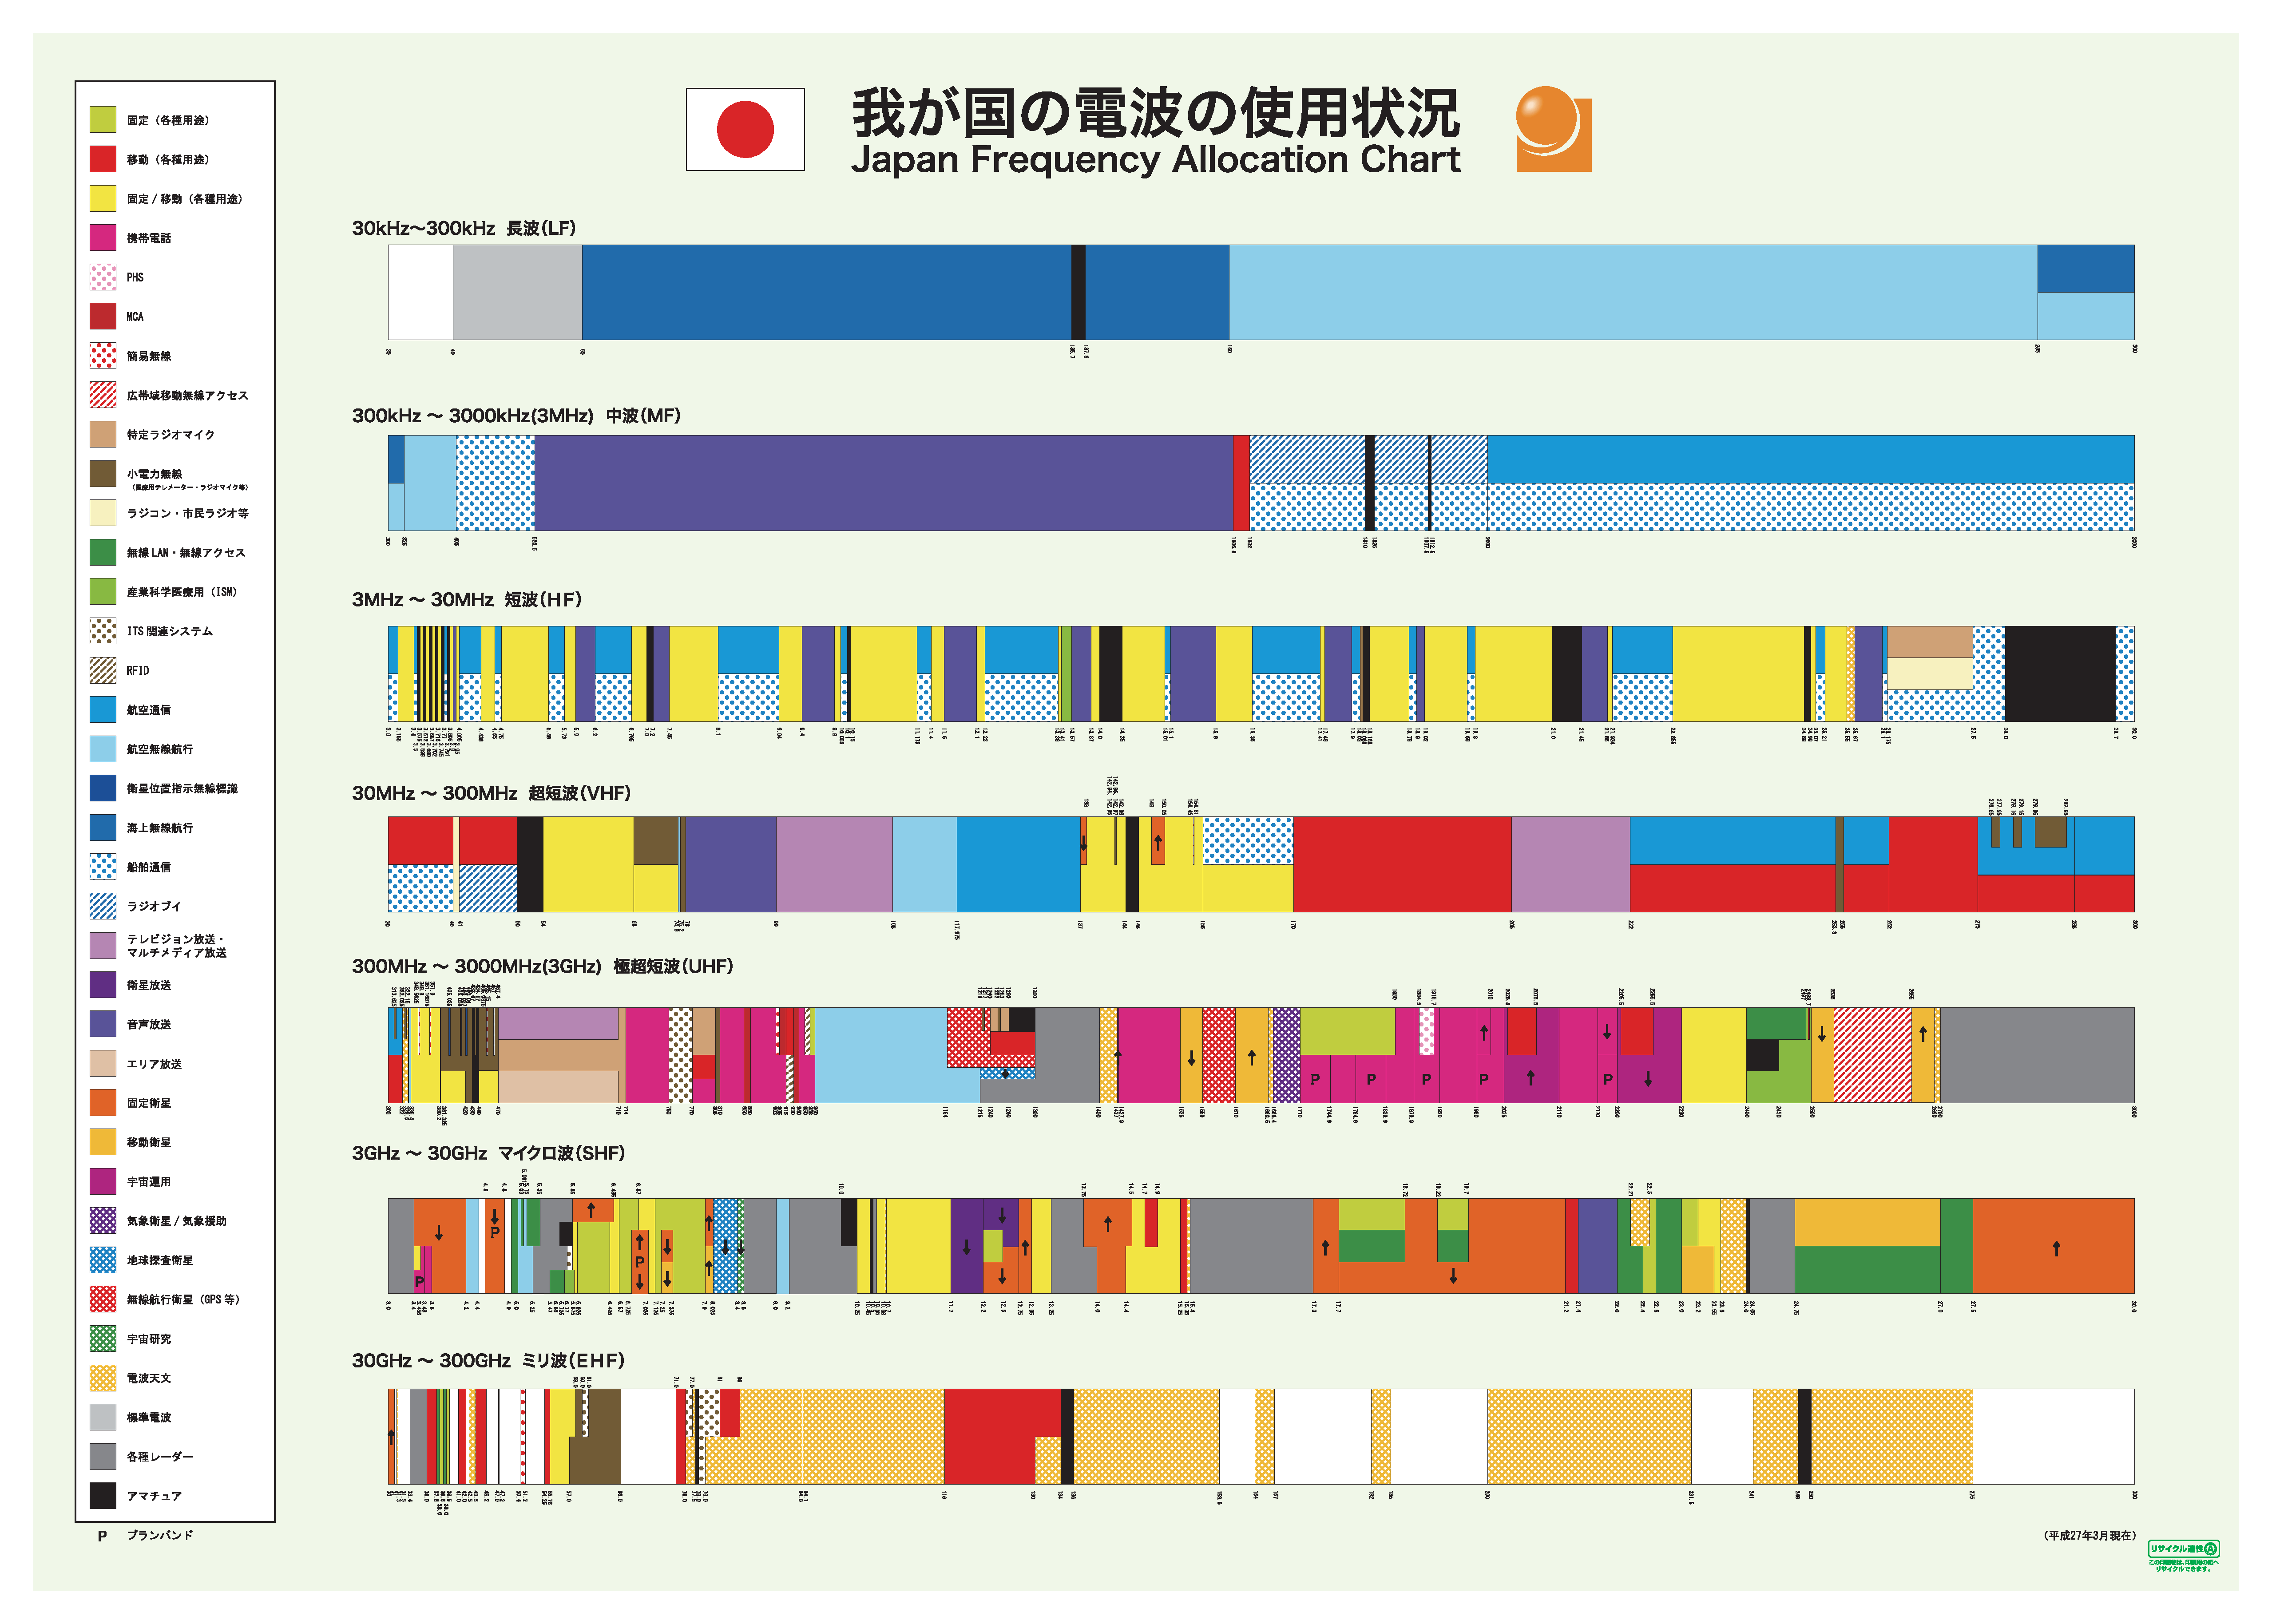
\includegraphics[width=150mm,clip]{frequency_alloc.pdf}
\caption{Japanese Frequency Allocation Chart.}
\label{fig:MIC}
\end{figure}

Since the finite spectrum resources are not able to fulfill the expoential growth of demand on traffic, it is necessary to review the present spectrum policy with fixed resource allocation for the next generation wireless communication sysytems and a effecient spectrum utilization turns to be a key problem. 

There are 2 main methods to ensure the bandwidth for new systems. Firstly, a spectrum arrangement on the whole wireless communication systems is utilized to extend available bandwidth. In 2011, an arrangement on television broadcasting is executed with switching to digital television broadcasing. However, it is not available for supporting the expoential growth of the data traffic and the number of systems. Second, an efficient and dynamic utilization method of bandwidth is considered to extend the probability for the future wireless communication systems, which is attracted attention as effective solution to the shortage of spectrum resources. 

According to the report \cite{ref:FCC} from Federal Communications Commission(FCC), actual spectrum usage on the licensed band is lack of balance in both temporal and spatial domain and instantaneous usage efficiency remains at 15\%~80\% even under crowd environment, such as urban areas, which means that an unused White Space(WS) exists even under temporal and spatial varying envrionment. However, it is not allowed to utilize White Space by other licensed or unlicensed systems based on current radio regulations.

\section{Spectrum Sharing Trend and Problem}
Cognitive Radio(CR)\cite{ref:Haykin} has been recognized as a promising solution to address the problem for improving the utilizetion of spectrum for various wireless applications. In a CR system from Fig.\ref{fig:CR_time} and \ref{fig:CR_space}, it allows the Secondary Users (SUs) to opportunistically utilize the temporal and/or spatial unused spectrum holes without causing interference to Primary Users (PUs). While SUs can occupy avaliable spectrum holes as long as the corresponding PU is inactive, they must immediately evacuate the band as soon as the corresponding PU appears.

\begin{figure}[!htp]
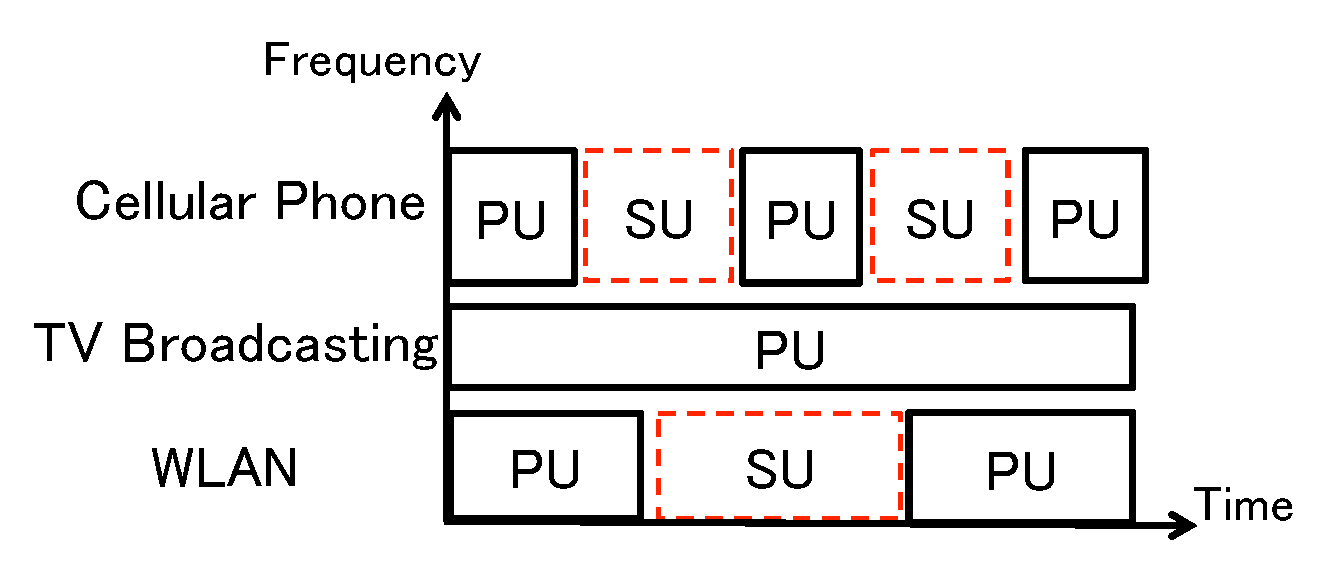
\includegraphics[width=150mm,clip]{CR_time.eps}
\caption{Coexsitance between PU and SU in time domain.}
\label{fig:CR_time}
\end{figure}

\begin{figure}[!htp]
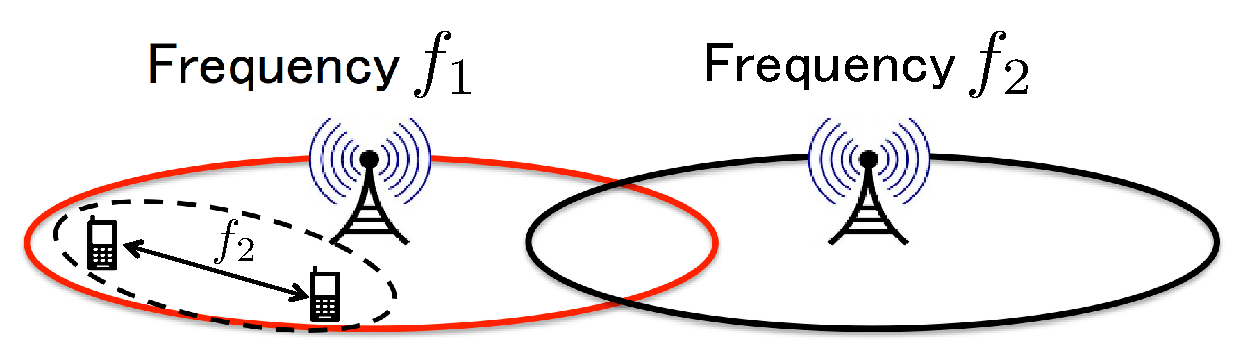
\includegraphics[width=150mm,clip]{CR_space.eps}
\caption{Coexsitance between PU and SU in space domain.}
\label{fig:CR_space}
\end{figure}

One of the main chanllenges is to intelligently determine ongoing PU activity to avoid interferece toward PU. SUs can evacuate the band without affecting PU’s activity and opportunistically access the spectrum to maximize the spectrum usage if the information about PU can be obtained in advance. Hence, more information about PU leads to more effective spectrum usage for SUs, and an external device for provding information of PU is necessary. One of the main chanllenges is to intelligently determine ongoing PU activity to avoid interferece toward PU. SUs can evacuate the band without affecting activity of PU and opportunistically access the spectrum to maximize the spectrum usage if the information about PU can be obtained in advance. Hence, more information about PU leads to more effective spectrum usage for SUs, and an external device for providing information of PU is necessary. However, it is difficult for SU to obtain the information about activity of PU individually according to the position of SU and it may leads a performation degradation on PU protection.

The idea of Spectrum Database has been studied for assisting SUs to effectively reuse the spectrum. SUs can access the database to obtain the surrounding radio environment information and optimize their own parameters,
such as modulation, transmitting power and so on. Federal Comminication Committee (FCC) has been considered a propagation model-based spectrum database to provide the spectrum available information whether the spectrum locating SU can be used or not [3]. The model-based database has to set a large margin to avoid interference to PU because the realistic radio environment with considering the effect of surrounding obstacles cannot be considered. Therefore, there is a limit to improve the spectrum utilization efficiency.

Authors in \cite{ref:Database1,ref:Database2,ref:Database3} proposed a measurement-based spectrum database as a realistic method. The measurement-based database generates the database information by gathering the measuring received power at SUs, which are inactive for communication. Then the real radio propagation situation can be known and more accurate information at SU location can be provided. Then, SUs access to the database with their own location information and download the responding average received signal power at the SU location as shown in Fig.\ref{fig:Database}.
\begin{figure}[!htp]
\begin{center}
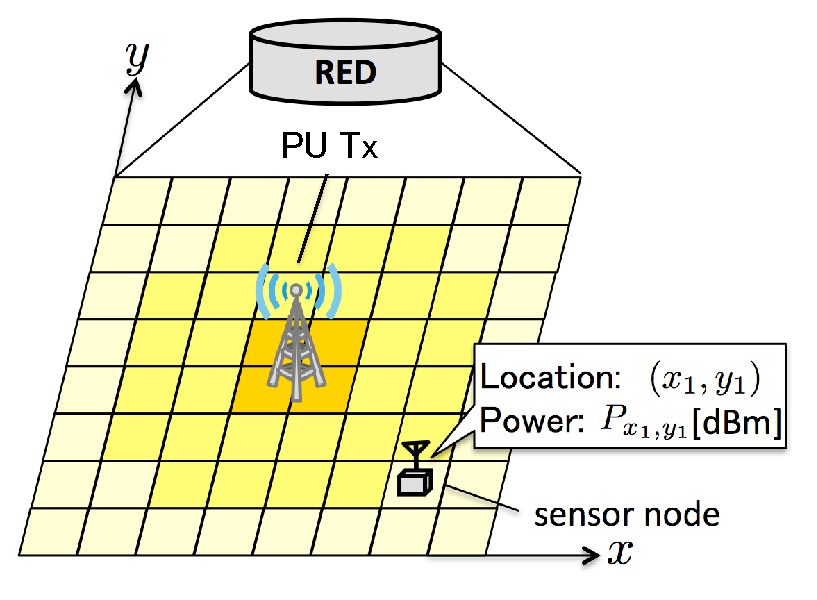
\includegraphics[width=120mm,clip]{database.eps}
\caption{Measurement-based Spectrum Database.}
\label{fig:Database}
\end{center}
\end{figure}

The database is constructed by using reported measurement results of averaged sampling value in each sensor node like energy detection spectrum sensing algorithm to calculate the average received signal power at each location. However, it is only appropriate under the assumption that the PU status is always ON. For example, in \cite{ref:ON1}\cite{ref:ON2}, the channel scenario is not considering primary user traffic during the sensing period. If there is a state transition from ON to OFF, sensor node will report the wrong received signal power to the database, which leads to low reliability and performance. Thus, it is necessary to detect PU’s state transition and extract the ON part only to the database to improve the reliability of database. In \cite{ref:quickest}, single status change of primary user is focused.

\section{Purpose}
In this thesis, we focus on a distribution transition between the ON status and OFF status, CUSUM (cumulative sum) algorithm \cite{ref:CUSUM} and GLR (Generalized Likelihood Ratio) algorithm \cite{ref:GLR} are used to detect the rise up point and rise down point, which is status change point from OFF to ON and ON to OFF. Finally, only ON power can be extracted with using the detected transition point and the sensing error reduction is possible. 

The remainder of this thesis is organized as follows. The overview of Cognitive Radio and Spctrum Sharing with Spectrum Database is introduced in Chapter \ref{chapter:CR}. In Chapter \ref{chapter:Database} the basic sensing method for calculating the reported information is presented as a measurement-based spcetrum database construction metrics and the problem of Spectrum database construction is described in detail. Chapter \ref{chapter:Propose} proposes the active period detection method of primary signal for spectrum database in detail and the simulation results and performance evaluation are discussed in Chapter \ref{chapter:Result} . Finally, Chapter \ref{chapter:Conclusion} concludes the thesis.



% Cognitive Radio ---
\chapter[CognitiveRadio]{Cognitive Radio}
%\addcontentsline{toc}{chapter}{Chapter 1\\Introduction}
\label{chapter:CR}
\pagenumbering{arabic}

\section{Overview of Cognitive Radio}

\section{Dynamic Spectrum Access for Spectrum Sharing}
    \subsection{Overlay Spectrum Sharing}
    \subsection{Underlay Spectrum Sharing}

\section{Overview of Spectrum Sharing with Spectrum Database}

% Spectrum Database ---
\chapter[Spectrum Database]{Spectrum Database}
%\addcontentsline{toc}{chapter}{Chapter 3\\Spectrum Database}
\label{chapter:Database}
In Chapter \ref{chapter:Database}, the overview of spectrum sharing with spectrum database and the measurement-based Spectrum Database proposed by our laboratory. And a problem of Spectrum Database Construction is described.

\section{Overview of Spectrum Sharing with Spectrum Database}
For further improving the performance for spectrum sharing, Federal Communications Commission(FCC), an independent agency of the United States government,proposed to fully utilize spectrum database for supporting spectrum sharing. Secondary User should obtain own postion by Global Position System(GPS) and access to database. FCC has already released the detailed rule of construction and managementfor TV broadcasting White Space and some service provider corporation have already established spectrum databases.\cite{ref:fcc,ref:google,ref:microsoft}. However, FCC-defined Database is determined by following a specified propagation model and only stores the decision information whether the White Space can be utilized or not at each position based on the calculation result from the propagation model. Based on the information from GPS, Secondary User accesses to the spectrum database to obtain the White Space information. Because interference towards Primary User is designed by managing geographic White Space conservatively, FCC-defined Spectrum Database is only treated as overlay spectrum sharing. Consequently, as the interference margin is set too large, the calculation of interfernce power with following a detailed propagation model is not considered, which is described in Chapter \ref{chapter:CR} that the spectrum usage efficiency improvement has a upper limit.


\section{Measurement-based Spectrum Database}
To obtain a large improvement on spectrum usage efficiency, underlay spectrum sharing spectrum database should be considered instead of overlay type. Thus, a more advanced radio environment database besides FCC-defined spectrum database is required for providing not only the White Space information, but also the information about Primary, such as Modulation and Coding Scheme(MCS) and transmision power, a more detailed propagation model, estimation error and the position of Primary receiver and so on.

    \subsection{Spectrum Datbase Construction based on Energy Detection}

\section{Problem of Spectrum Database Construction }


% proposed method ---
% proposed method ---
\chapter[Active Period Detection Method of Primary Signal for Spectrum Database]{Proposed Method}
\label{chapter:Propose}
\section{System model}
\label{system}

We assume that a sensor node tunes to a frequency band and obtains samples ${\bf y}=\left\{y[1],y[2],...,y[N]\right\}$ from a primary transmitter. $N$ is the sample number during the sensing period. Since a multiple ON/OFF environment is considered, the sensing samples ${\boldmath y}$ is shown in Fig. 2 as follows

\begin{eqnarray}
y[i] = 
\begin{cases}
\;n[i],    i=1,...\tau_1-1 \\ \nonumber
\; \\ \nonumber
\;x[i]+n[i], i=\tau_1,...,\tau_2-1 \\
\; \\ \nonumber
\;n[i],    i=\tau_2,..,N,
\end{cases}
\end{eqnarray}

where $\tau_1$ and $\tau_2$ is the rise up point at which primary user starts to transmit and rise down point at which primary user stop transmitting respectively. If $\tau_1=1$ and $\tau_2=N$, the primary user is always transmitting during the sensing period. On the other hand, if $\tau_1=1$ and $\tau_2=1$, the primary user is not at present during the sensing period. In this paper, we consider only the primary user starts and stops transmission during the sensing period.
If the primary user is not transmitting, $y[i] = n[i]$, in which $n[i]$ is Addative White Gaussian Noise with mean 0 and variance $\sigma^2$. If the primary user starts transmitting, then $y[i] = x[i] + n[i]$, in which $x[i] = gs[i]$. $g$ is the channel gain and the $s[i]$ is the signal of the primary user. Therefore, we assume $x[i]$ is white and Gaussian with mean 0 and variance $P$. $P$ depends on the channel gain and the transmitter power of the primary user. In the wireless environment, the signal of the primary experiences pathloss and shadowing and  multipath fading, so the value of $P$ is not possible to be known accurately by the sensor. Thus, as a solution to received power detection problem, a transition point detection algorithm is considered. 

\section{Transition Point Detection Method under Multiple ON/OFF Environment }    

In this section, transition point detection algorithm for the status of primary user is introduced in detail. As the Fig. \ref{system_model} is shown, the sample of the ON and OFF status follows a Gaussian distribution $\mathcal{N}(0,\sigma^2+P)$ and $\mathcal{N}(0,\sigma^2)$ respectively. The probability density function(PDF) follows the eq. (\ref{normal}) is given by

\begin{eqnarray}
\begin{cases}
\;f_0(t) = \frac{1}{\sqrt{2\pi\sigma^2}} \rm{exp}^{-\frac{t^2}{2\sigma^2}} \\
\; \\ \nonumber
\;f_1(t) = \frac{1}{\sqrt{2\pi(\sigma^2+P)}} \rm{exp}^{-\frac{t^2}{2(\sigma^2+P)}}.
\end{cases}
\label{normal}
\end{eqnarray}

\begin{center}
  \begin{figure}[t]
    \centering
    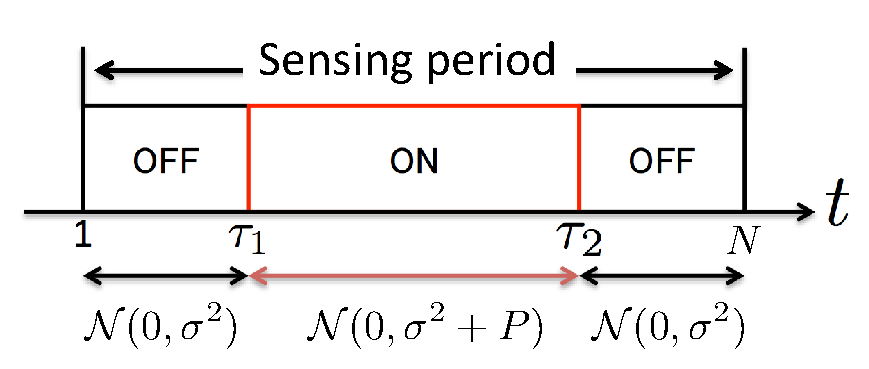
\includegraphics[width=90mm]{systemodel.eps}
    \label{system_model}
    \caption{\normalsize{System model.}}
  \end{figure}
\end{center} 

\subsection{CUSUM algorithm}
The cumulative sum (CUSUM) algorithm, which was first proposed by Page in \cite{ref:CUSUM}, is used to detection the transition point when $P$ and $\sigma^2$ is assumed to be known.
The PDF $f_0(t)$ and $f_1(t)$ are fully specified. Thus, the log probability density ratio $l(y[i])$ is also fully defined by the eq. (\ref{like1}) and (\ref{like2}),

\begin{eqnarray}
l_{0}(y[i]) &=& {\rm ln}\left\{\frac{f_0(y[i])}{f_1(y[i])}\right\} \label{like1} \\ 
&=& -\frac{2(P+\sigma^2)\sigma^2}{Py^2[i]} + \frac{1}{2}{\rm ln}\left\{\frac{P+\sigma^2}{\sigma^2}\right\}, \nonumber
\end{eqnarray}

\begin{eqnarray}
l_{1}(y[i]) &=& {\rm ln}\left\{\frac{f_1(y[i])}{f_0(y[i])}\right\} \label{like2} \\ 
&=& \frac{Py^2[i]}{2(P+\sigma^2)\sigma^2} + \frac{1}{2}{\rm ln}\left\{\frac{\sigma^2}{P+\sigma^2}\right\}. \nonumber
\end{eqnarray}

When the primary user is on the OFF and ON status, the average log probability density ratio can be calculated respectively using the eq. (\ref{D_f0}) and (\ref{D_f1}),
\begin{eqnarray}
E_{f_0}\left\{l_0(y[i])\right\} &=& -\int f_0(y){\rm ln}\left\{\frac{f_0(y)}{f_1(y)}\right\}dy \nonumber \\ 
&=&-D(f_0||f_1)\leq 0, \label{D_f0} 
\end{eqnarray}
\begin{eqnarray}
E_{f_1}\left\{l_1(y[i])\right\} &=& \int f_1(y){\rm ln}\left\{\frac{f_1(y)}{f_0(y)}\right\}dy \nonumber \\
&=& D(f_1||f_0)\geq 0 \label{D_f1},
\end{eqnarray}
where $D(f_0||f_1)$ is the Kullback-Leibler divergence of $f_0$ from $f_1$ and $D(f_1||f_0)$ vice versa, which is shown in eq. (\ref{KL})
\begin{eqnarray}
D(f_0||f_1)=\frac{P}{2(P+\sigma^2)}+\frac{1}{2}{\rm ln}\left\{\frac{\sigma^2}{\sigma^2+P}\right\}.
\label{KL}
\end{eqnarray}
Hence, when the primary user is at present, which means the sample before primary user changes its status from OFF to ON, the probability density ratio $l(y)$ has a negative trend. After a change point from ON to OFF, $l(y)$ has a positive trend.
Using the characterics discussed above, an algorithm for detecting a status transition (ON$\rightarrow$OFF or OFF$\rightarrow$ON) of the primary user can be defined as comparing,  
\begin{eqnarray}
g_t =  \max_{k \leq t}\left\{\sum_{i=1}^tl(y[i]-\sum_{i=1}^kl(y[i]))\right\}=\max_{k \leq t}\sum_{i=k+1}^tl(y[i]),
\label{Cusum}
\end{eqnarray}
with a threshold $h$. If $g_t$ is larger than $h$, the existence of the primary user is declared. Since $l(y)$ has a positive trend during the ON status of the primary.

\begin{figure}[t]
\centering
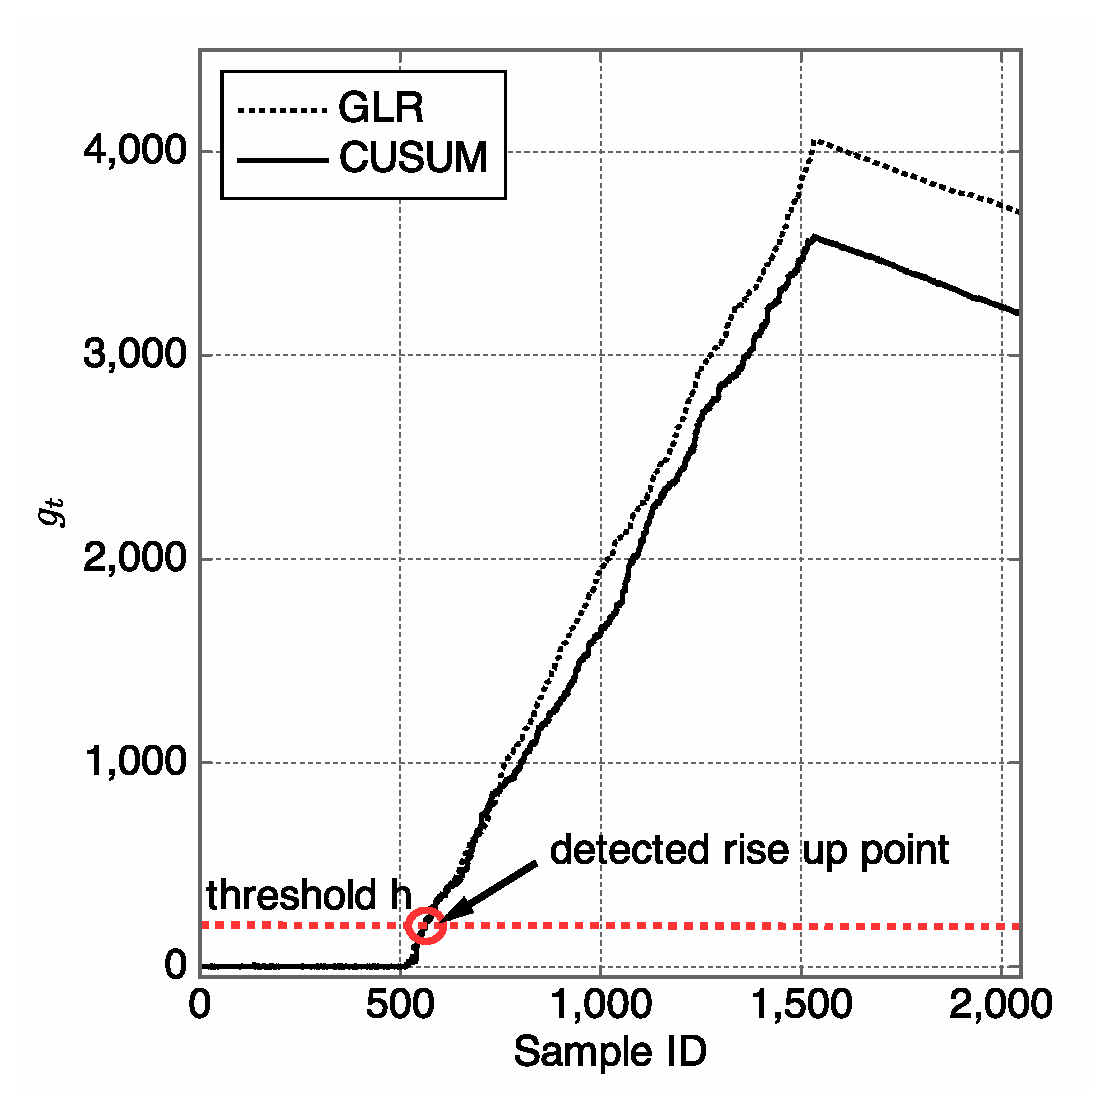
\includegraphics[width=87mm]{OFF2ON.eps}
\caption{ Statistic $g_t$ using the probability density ratio $l_0(y)$  when the rise up point is 512th sample and the rise down point is 1532th sample.}
\label{OFF2ON}
\end{figure}

Also, the eq. (\ref{Cusum}) can be written as
\begin{eqnarray}
g_{t+1} &=& \max_{k \leq t+1}\left\{\sum_{i=k+1}^{t+1}l(y[i])\right\} \nonumber \\ 
&=& \max\left\{\max_{k \leq t+1}\left\{\sum_{i=k+1}^{t+1}l(y[i])\right\},0\right\} \nonumber \\
&=& \max\left\{\max_{k \leq t+1}\left\{\sum_{i=k+1}^{t+1}l(y[i])\right\}+l(y[i]),0\right\} \nonumber \\
&=& \left\{g_t+l(y[t+1])\right\}^{+}.
\label{rec}
\end{eqnarray}
$\left\{.\right\}^{+}$means that the value must be postive. Hence, $g_t$ can be computed recursively by setting $g_0=0$. To sum up, the CUSUM algorithm works as the following process:
\begin{enumerate}
  \item[i]. compute $l(y)$ for each sample using eq. (\ref{like1}) or (\ref{like2}).
  \item[ii]. compute the statistic $g_t$ using eq. (\ref{rec}).
  \item[iii]. compare the statistic $g_t$ with a threshold $h$.
  \item[iv]. If $g_t \geq h$, the existence of the primary user is declared.
\end{enumerate}

\subsection{GLR algorithm}
In realistic wireless channels, the exact value of $P$ is difficult to be known exactly. It is more reasonable to assume that $P$ belongs to a range, that is $P\in[P_{{\rm min}}, P_{\rm {max}}]$. In this case, a generalized likelihood ratio(GLR) algorithm\cite{ref:GLR} for transition point detection is applied. Since the value of $P$ is unknown, the statistic $g_t$ is defined as the following eq. (\ref{Glr}),
\begin{eqnarray}
g_t &=& \max_{k \leq t}\left\{ \sum_{i=k+1}^tl(y[i])\right\}={\rm ln}\left\{\prod_{i=k+1}^k\frac{f_{1,P}(y[i])}{f_0(y[i])}\right\} \nonumber \\ 
   &=& \max_{k \leq t}\left\{\sum_{i=k+1}^t\left\{ \frac{Py^2[i]}{2(P+\sigma^2)\sigma^2}+\frac{1}{2} {\rm ln}(\frac{\sigma^2}{P+\sigma^2}) \right\}\right\},
\label{Glr}
\end{eqnarray}
\begin{figure}[t]
\centering
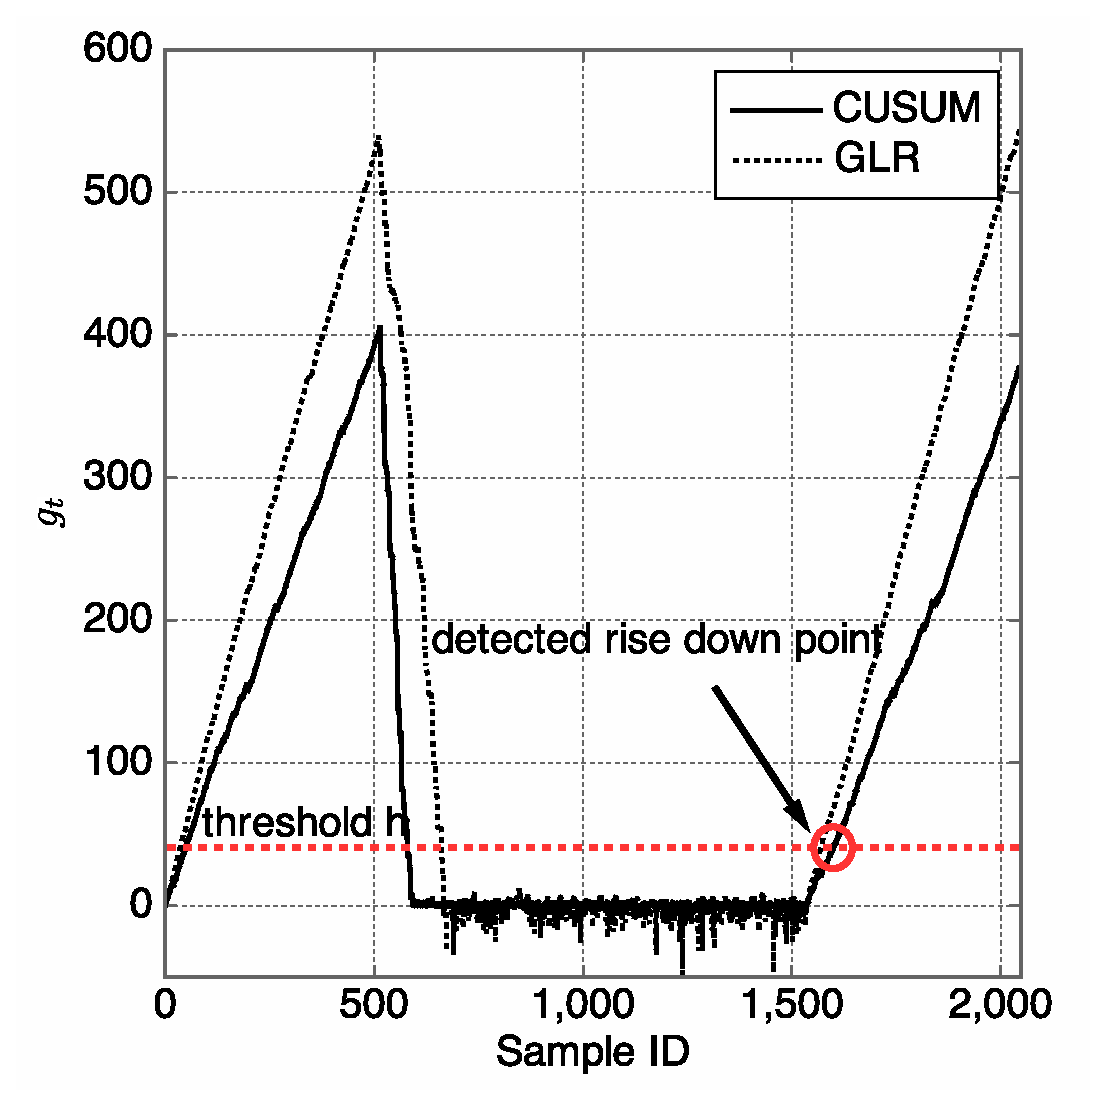
\includegraphics[width=87mm]{ON2OFF.eps}
\caption{Statistic $g_t$ using the probability density ratio $l_1(y)$ when the raise up point is 512th sample and the raise down point is 1532th sample.}
\label{ON2OFF}
\end{figure}
where $f_{1,P}(t)$ is the probability density function of the received signal when the varinace of the signal part is $P$. Therefore a function $f(P)$ defined as eq. (\ref{fp}) is used to calculate the statistic $g_t$,
\begin{eqnarray}
f(P) &=& \sum_{i=k+1}^t\left\{ \frac{Py^2[i]}{2(P+\sigma^2)\sigma^2}+\frac{1}{2} {\rm ln}(\frac{\sigma^2}{P+\sigma^2})\right\} \nonumber\\ 
&=&\frac{P}{2(P+\sigma^2)\sigma^2}\hat{y}+(t-k)\frac{1}{2}{\rm ln}\left\{ \frac{\sigma^2}{P+\sigma^2} \right\},
\label{fp}
\end{eqnarray}
where $\hat{y}=\sum_{i=k+1}^t y[i]$. To find a the power $P^{*}$ that maximizes the function $f(P)$ over $P \in [P_{{\rm min}}, P_{{\rm max}}]$, it can be calculated as below,

\begin{equation}
P^{*}=
\left\{
\begin{array}{ll}
P_{{\rm max}}, & (t-k)\leq\frac{\hat{y}}{P_{{\rm max}}+\sigma^2}, \\
\\ \nonumber
\frac{\hat{y}}{t-k}-\sigma^2, & \frac{\hat{y}}{P_{{\rm max}}+\sigma^2}\leq(t-k)\leq\frac{\hat{y}}{P_{{\rm min}}+\sigma^2}, \\
\\ \nonumber
P_{{\rm min}}, & (t-k) \geq \frac{\hat{y}}{P_{{\rm min}}+\sigma^2}.
\end{array}
\right.
\label{maxP}
\end{equation}

As same as the CUSUM algorithm, in the GLR algorithm the statistic value $g_t$ is calculated in eq. (\ref{Glr}) with choosing the a power $P^{*}$ from the equation (\ref{maxP}), and is compared with the threshold $h$. Once $g_t>h$, the existance of the primary user is declared.

\subsection{Threshold configuration for CUSUM and GLR algorithm}
To set a threshold for the transition point detection, we first assume $t_0$ denotes the time when the statistic $g_t$ exceeds the threshold $h$, and define $\bar{T_0}=E[t_0]$ is the mean time to a false alarm. Following \cite{ref:threshold_cusum} and \cite{ref:threshold_GLR}, some simple bounds on $\bar{T_0}$ can be derived.

For CUSUM algorithm, the relationship between the mean false alarm and threshold is as follows.
\begin{eqnarray}
\bar{T_0} \geq e^h.
\end{eqnarray}
For GLR algorithm, the threshold is set to be $h=-{\rm ln}\left\{\frac{a}{b}\right\}$ , where 
\begin{eqnarray}
b=3{\rm ln}\left\{a^{-1}(1+\frac{1}{D(f_1,P_{min}||f_0)})^2\right\},
\end{eqnarray}
and $a$ follows the following inequality.
\begin{eqnarray}
\bar{T_0} \geq \frac{1}{a}.
\end{eqnarray}

% simmulation
\chapter[Simulation]{Simulation}
\label{chapter:Result}

%\section{System Model}

%\section{Simulation Results}

\section{Performance evaluation}
In this section, we use computer simulation to evaluate the performance of transition point detection and the received power detection using CUSUM and GLR algorithm. The simulation parameters are shown in Table \ref{parameter}.

\begin{table}[!htp]
\begin{center}
 \caption{\normalsize{Simulation parameters}}
 
\normalsize

  \begin{tabular}{c|c}
    & \\
    Parameter &Value \\ \hline
    SNR & 0〜20[dB] \\
    $[P_{{\rm min}},P_{{\rm max}}]$ & [$P$/2, 2$P$] \\
    $\sigma^2$ & 1 \\
    sample number & 2048 \\
    $\bar{T}_0$ & 10 \\
    transition partern & OFF $\rightarrow$ ON $\rightarrow$ OFF \\
    rise up point & 512th sample\\
    rise down point & 1536th sample\\
    Number of trials & 10,000 \\ \hline
  \end{tabular}
\label{parameter}
\end{center}
\end{table}

To vertify the performance of the received power, we evalate

\begin{enumerate}
\item the performance of the rise up point and the rise down point detection, 
\item the CDF(Cumulative Distribution Function) of transition point.
\item the performance of the received power detection using the detected transition point.
\item the power difference in different ON percentage of primary user.
\end{enumerate}

\section{Simulation results}
Figures \ref{transition_up} and \ref{transition_down} show the boxplot results of detected rise up point and rise down point respectively. The body of the boxplot consists of a box, which goes from the fisrt quartile to the third quartile. The line drawn at the box means the median of the detected transition point. The lines extended from the box called whiskers mean the smallest and the largest nonoutlier from the box. The real rise up point and rise down piont are fix on the 512th sample and 1532th sample. From the simulation results, we can see that in low SNR region the variation of transition point is large, howerver, in high SNR region the detected transition point converges to the real one.

Figures \ref{Powdiff} shows the performance of the power difference with the real power. 
The received power detection without considering ON/OFF transition during the sensing period, which means the all samples is used for calculating the received power, is considered as a conventional method for comparison. The dotted line means that the ideal case that the real received power is detected exactly. The power difference $P_{\rm diff}$ with real power is defined as follows,
\begin{eqnarray}
P_{{\rm diff}} &= P-P_{{\rm ON}}.
\label{diff}
\end{eqnarray}

Fig.\ref{cdf_off2on} and \ref{cdf_on2off} shows the cdf results of detected rise up point and rise down point. It is obvious that a higher detection probability on the real transition point can be gained  when SNR=10 [dB] than SNR=0[dB], because noise effect is low to the CUSUM algorithm and GLR algorithm and peak detection when SNR is in high region

The simulation result shows that the active period detection using CUSUM algorithm and GLR algorithm and peak detection can obtain a better performance than the conventional method. In low SNR region, power difference of the proposed method can achieve 0.5[dB] gain than that of the conventional one, and in high SNR region, 1.3[dB] is improved. It can be considered that a noise effect is low to propose method and the transition point is detected more accurate in high SNR region than in low SNR region.

Fig.\ref{per} shows the power difference with the real power at different ON percentage during the sensing period. At this time, 25\%, 50\%, 75\% is evaluated. It is clear that longer time of primary user occupies during the sensing period, lower power different can be gained with proposed method.  

\begin{figure}[!htp]
\centering
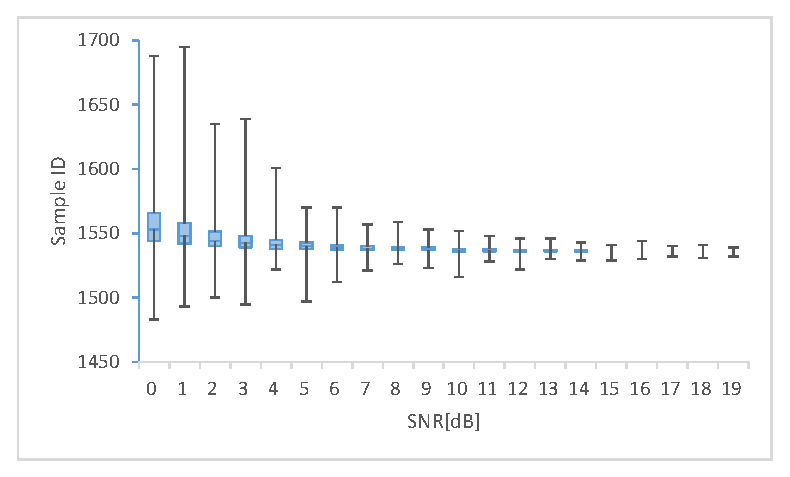
\includegraphics[width=120mm]{transition_up.eps}
\caption{Boxplot result of the rise up point.}
\label{transition_up}
\end{figure}
\begin{figure}[!htp]
\centering
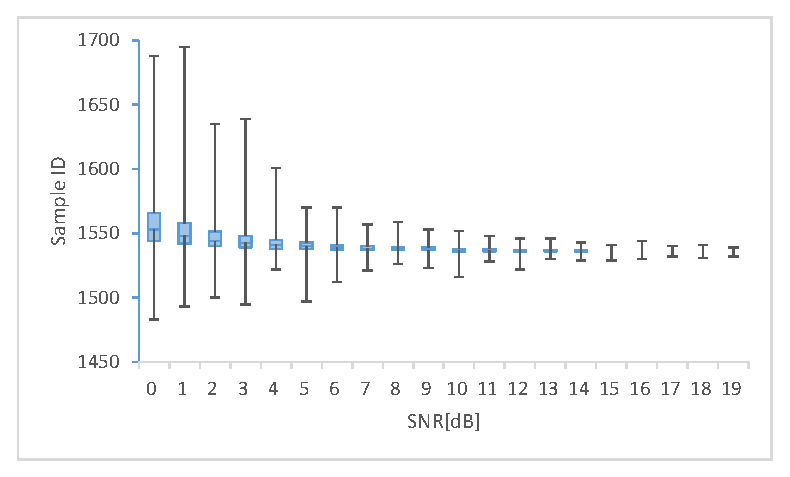
\includegraphics[width=120mm]{transition_down.eps}
\caption{Boxplot result of the rise down point.}
\label{transition_down}
\end{figure}

\begin{figure}[!htp]
\centering
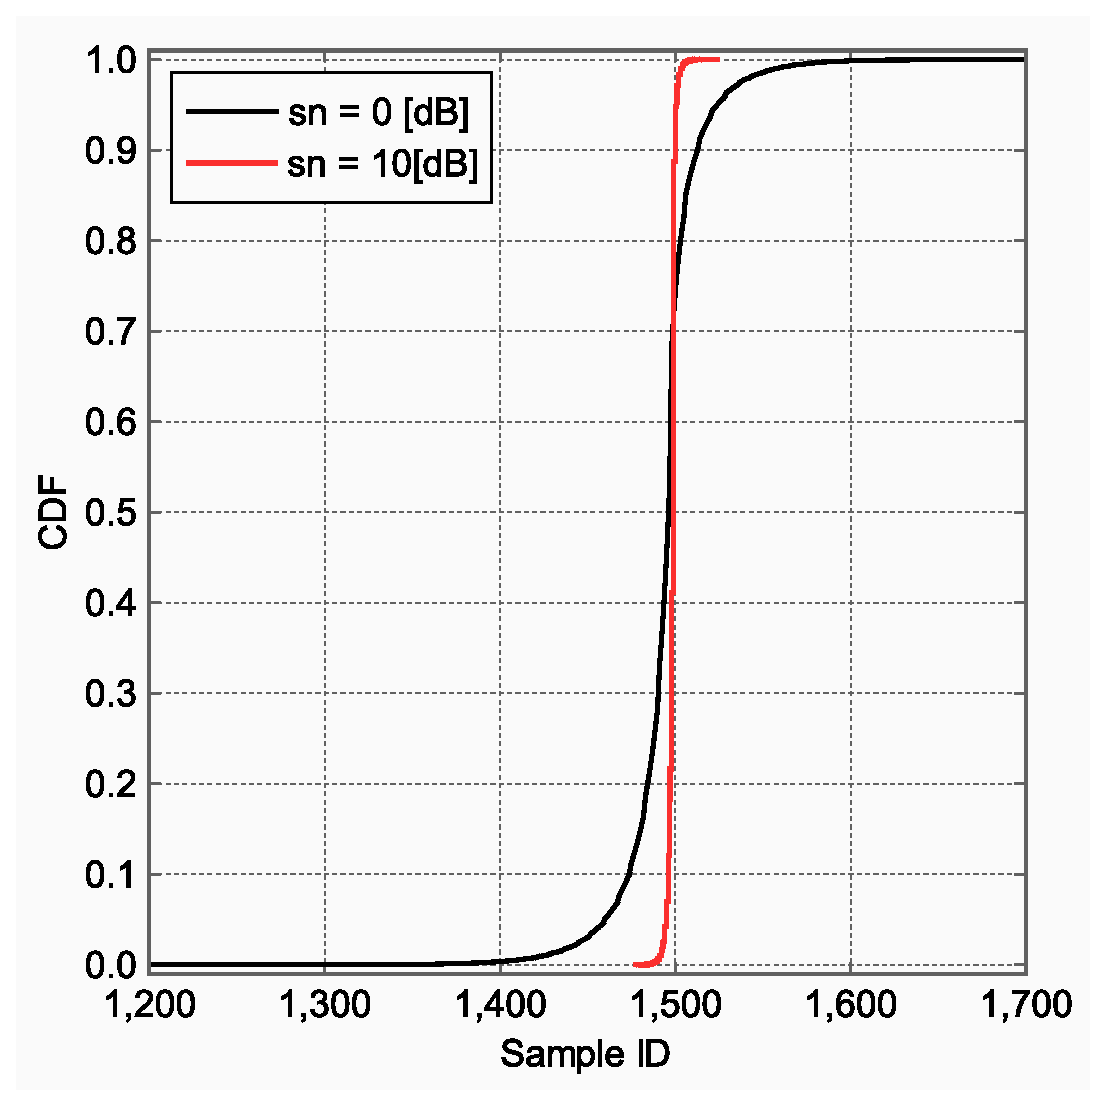
\includegraphics[width=100mm]{cdf_OFF2ON.eps}
\caption{CDF of rise up point detection(rise up point is set to be 500th sample).}
\label{cdf_off2on}
\end{figure}


\begin{figure}[!htp]
\centering
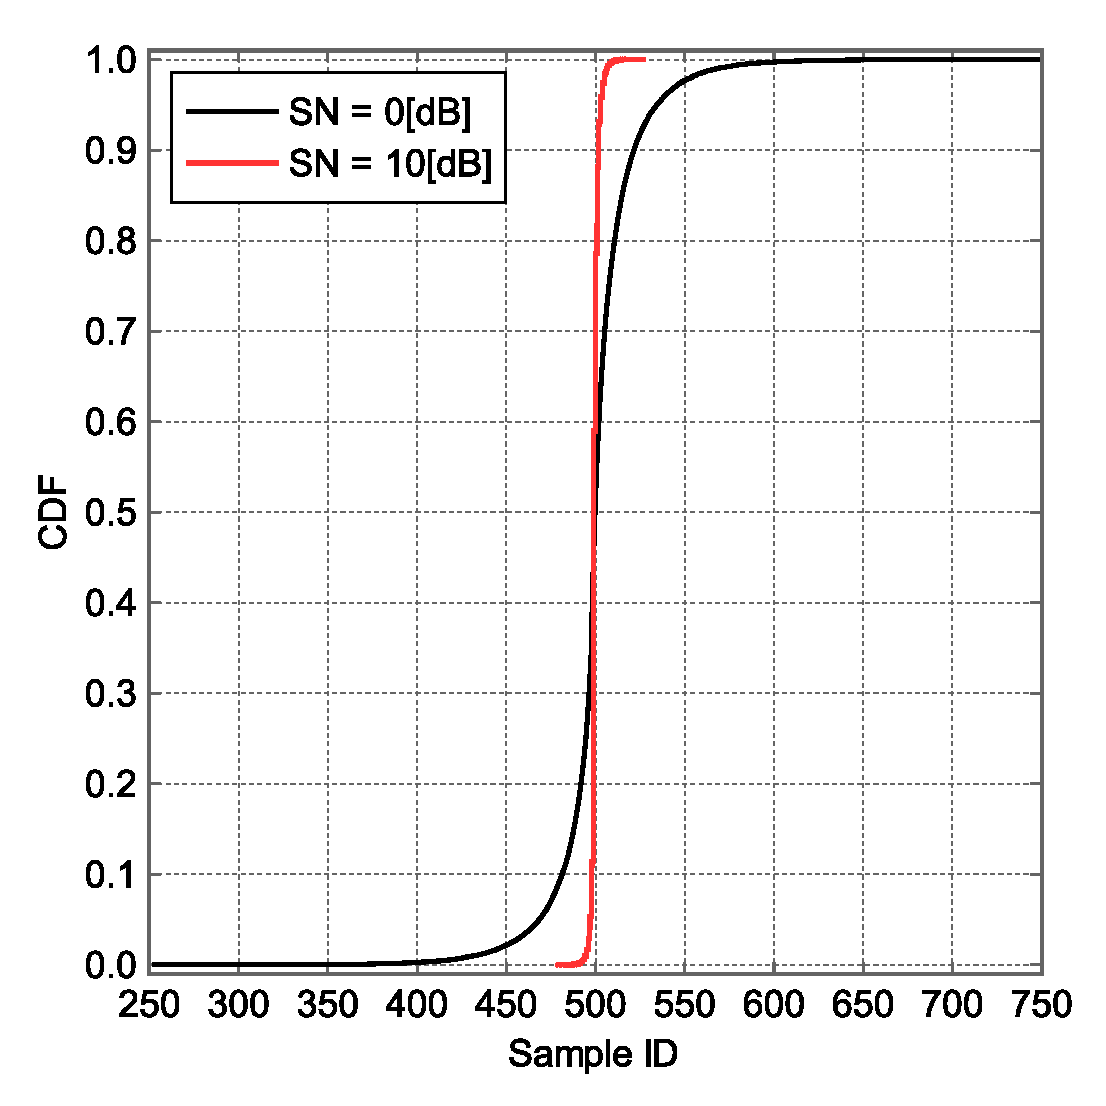
\includegraphics[width=100mm]{cdf_ON2OFF.eps}
\caption{CDF of rise down point detection(risen down point is set to be 1500th sample).}
\label{cdf_on2off}
\end{figure}

\begin{figure}[!htp]
\centering
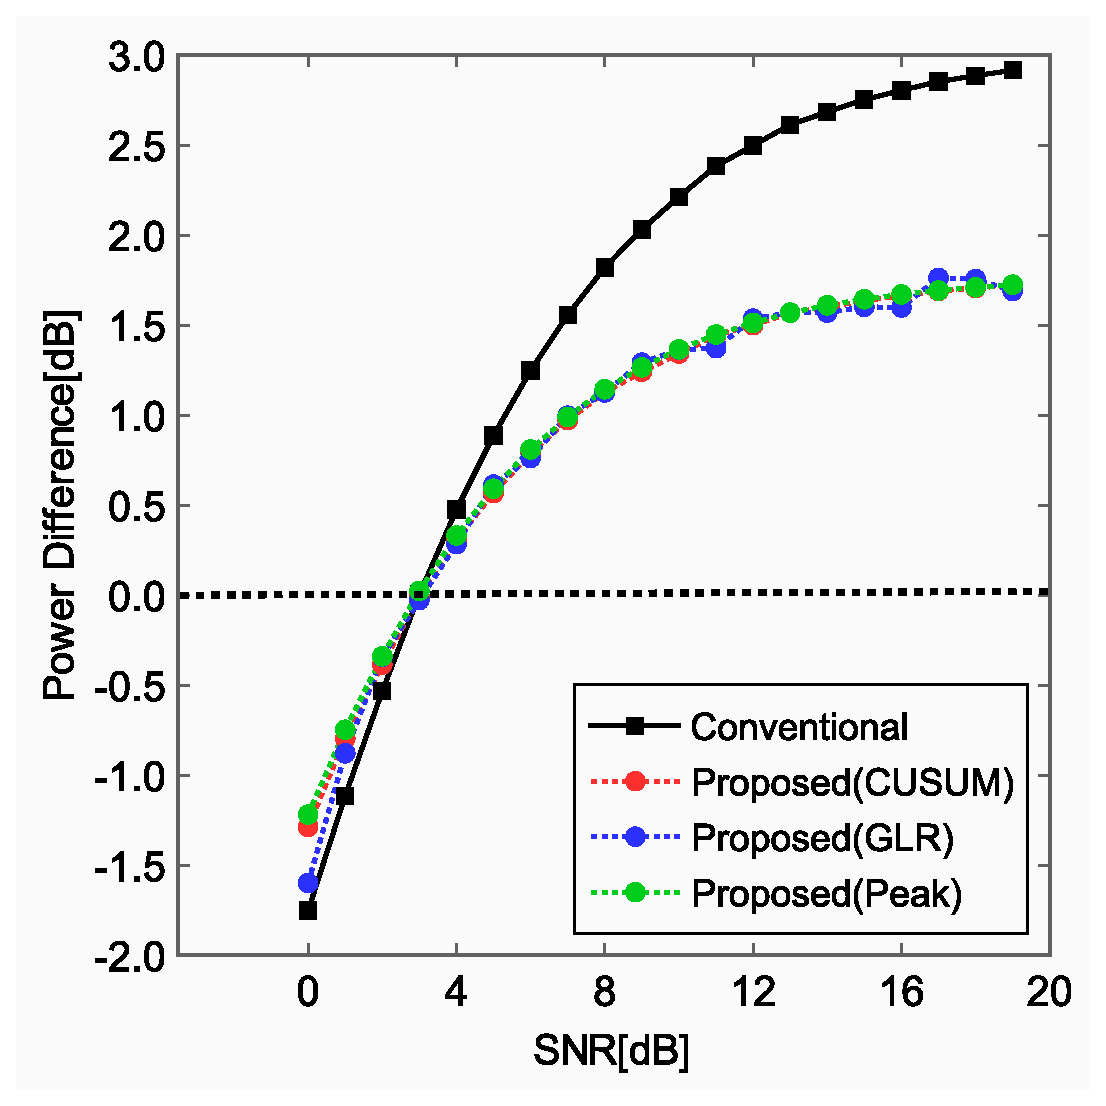
\includegraphics[width=100mm]{peak.eps}
\caption{The power difference with the real power.}
\label{Powdiff}
\end{figure}

\begin{figure}[!htp]
\centering
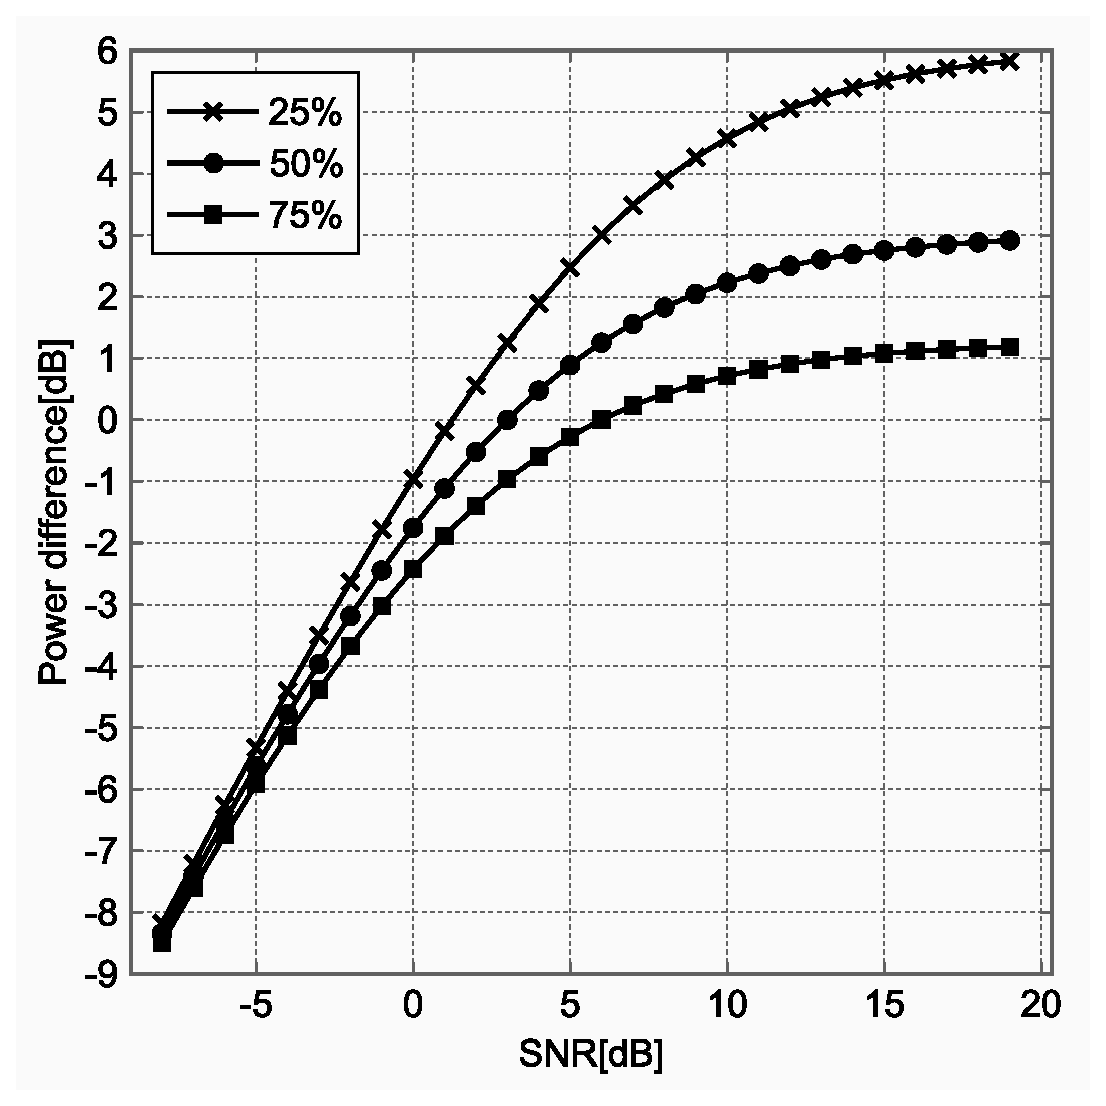
\includegraphics[width=100mm]{per.eps}
\caption{The power difference with the real power at different ON percentage during the sensing period.}
\label{per}
\end{figure}

% conclusion ----
\chapter[Conclusion]{Conclusion}
\label{chapter:Conclusion}

In this paper, as a solution to the sensing error under multiple ON/OFF environment for Spectrum Database, a transition point detection algorithm is applied for the received power detection. Based on the detected transition point of the primary user status by using CUSUM algorithm and GLR algorithm. an active period of the primary user can be extracted. Transition point is well-detected and an improvement of sensing error can be confirmed through simulation results.



% list of figure/tables
% \listoffigures
% \listoftables
%\bibliographystyle{}	% bib style
%\bibliography{}	% your bib database

\begin{acknowledgments}
\addcontentsline{toc}{chapter}{Acknowledgement}
\end{acknowledgments}

\begin{thebibliography}{99}
\addcontentsline{toc}{chapter}{References}
\bibitem{ref:CR}J. Mitola III and G. Q. Maguire, Jr., ``Cognitive radio: making software radios more personal,'' IEEE Personal Communications, vol. 6, no. 4, pp. 13–18, Aug. 1999.
\bibitem{ref:Haykin} S. Haykin, ``Cognitive radio: Brain-empowered wireless communications,'' {\it IEEE J.Selected Areas Commun.},vol. 23, no. 2, pp. 201 - 220, Feb. 2005.
\bibitem{ref:FCC}Federal Communications Commission, SECOND MEMORANDUM OPINION AND ORDER, Sept. 2010.
\bibitem{ref:Database1}H. Rajib, K. Inage, M. Ohta, T. Fujii,“Measurement based radio environment database using spectrum sensing in cognitive radio, ”Proc. iCOST 2011, Shanghai, Oct. 2011.
\bibitem{ref:Database2}T. Fujii,K. Inage,M. Kitamura, O. Altintas, H. Kremo, H.Tanaka, "Probing the spectrum with vehicles: towards an advanced spectrum database", IEEE VNC 2013, Dec. 2013.
\bibitem{ref:Database3}M. Kitamura, K. Inage, Y. Ohue, T. Fujii, "Development of measurement based spectrum database for efficient spectrum sharing, "SDR-WInncomm2014, Illinois, USA, Mar. 2014.
\bibitem{ref:ON1}G. Zhou, J. Wu, K. Sohraby, ”Cooperative Spectrum Sensing with a Progressive MAP Detection Algorithm,” Proc. GLOBECOM, pp.1-5, Dec. 2011.
\bibitem{ref:ON2}Y. Pei; Y. Liang, K.C.Teh, K. H. Li, ”Sensing-throughput tradeoff for cognitive radio networks: A multiple-channel sceario,” Proc. IEEE PIMRC, pp.1257-1261, 13-16 Sept. 2009.
\bibitem{ref:quickest}L.Lai, Y.Fan, and H.V.Poor,“ Quickest Detection in Cognitive Radio: A Sequential Change Detection Framework, ” Proc. IEEE Globecom, Dec. 2008.
\bibitem{ref:CUSUM}E. Page, "Continuous inspection schemes," {\it Biometrika}, vol. 41, pp. 100-115, 1954.
\bibitem{ref:GLR}G. Lorden, "Procedures for reacting to a change in distribution," {\it Annals of Mathematical Statistics}, vol. 42, no. 6, pp. 1897-1908, 1971.  
\bibitem{ref:threshold_cusum}G. Lorden, "ON excess over the boundary," {\it Annals of Mathematical Statistics}, vol. 41, pp.520-527, Apr. 1970.
\bibitem{ref:threshold_GLR}G. Lorden, "Open-ended tests for Koopman-Darmois families," {\it Annals of Statistics}, vol. 1, no. 4, pp. 520-527, Apr. 1970.
\end{thebibliography}

\begin{publication}
  \addcontentsline{toc}{chapter}{Publications}
{\bf International Conference Papers}
  \begin{enumerate}[{}i{.}]
    %\setlength{\itemsep}{-1mm}
  
      \item \underline{Hao Wang}, Takeo Fujii, "Transition detection with Spectrum Database using Weighted Cooperative Sensing," Proc IEEE ICUFN, July. 2014.
 
      \item \underline{Hao Wang}, Takeo Fujii, "Active Period Detection Method of Primary Signal for Radio Environment Database," SmartCom2015, SR2015-50, pp. 21-22 , Oct. 2015.
      \item \underline{Hao Wang}, Koya Sato, Takeo Fujii, "Received Power Detection under Multiple ON/OFF Environment for Registering Radio Environment Database," Proc IEEE ICTC, Oct. 2015.
 
      \item Koji Ichikawa, \underline{Hao Wang}, Koya Sato, Takeo Fujii, "Height Power Estimation with Radio Environment Database in Urban Area," Proc IEEE IFUCN, July. 2015.
   \end{enumerate}
{\bf Domestic Conference Papers}
    \begin{enumerate}[{}i{.}]
        \item \underline{王昊}, 中川洸佑, 北村優行, 藤井威生, "重み付け協調センシングを用いた無線環境データベ ースによる状態遷移検出法," 信学総大, B-17-19, March 2016.
         \item \underline{王昊}, 藤井威生, "重み付け協調センシング及び電波環境データベースを用いたプライマリユーザの状態遷移検出法の一検討," 信学技報SR2015-1, pp. 1-6, May 2015.
         \item 市川浩次, \underline{王昊}, 佐藤光哉, 藤井威生, "市街地環境における電波環境データベース連携による高さ方向の信号電力推定," 信学技報SR2015-2, pp. 7-12, May 2015.
         \item \underline{王昊}, 佐藤光哉, 藤井威生, "フェージング環境におけるプライマリユーザ信号の時間的変化を考慮したデータベース精度向上法の検討," 信学技報SR, March 2016.(発表予定)
         \item 長谷川嶺, \underline{王昊}, 藤井威生, "電波環境データベース精度向上のための観測データクラスタリング法," 信学総大, B-17-19, March 2016.(発表予定)
    \end{enumerate}

\end{publication}

\begin{appendix}
\addcontentsline{toc}{chapter}{Appendix}
From the next page, the program source is attached. 
\end{appendix}


\end{document}
